\documentclass[conference]{IEEEtran}
\IEEEoverridecommandlockouts
% The preceding line is only needed to identify funding in the first footnote. If that is unneeded, please comment it out.
\usepackage{cite}
\usepackage{amsmath,amssymb,amsfonts}
\usepackage{algorithmic}
\usepackage{graphicx}
\usepackage{textcomp}
\usepackage{xcolor}
\usepackage[brazilian]{babel}
\usepackage[utf8]{inputenc}
\usepackage[T1]{fontenc}
\def\BibTeX{{\rm B\kern-.05em{\sc i\kern-.025em b}\kern-.08em
    T\kern-.1667em\lower.7ex\hbox{E}\kern-.125emX}}

\graphicspath{{img/}}
\begin{document}

\title{Bancos de Dados em Grafos\\
%{\footnotesize \textsuperscript{*}Note: Sub-titles are not captured in Xplore and
%should not be used}
%\thanks{Identify applicable funding agency here. If none, delete this.}
}

\author{\IEEEauthorblockN{Gustavo Estrela de Matos}
\IEEEauthorblockA{\textit{Instituto de Matemática e Estatísticas} \\
\textit{Universidade de São Paulo}\\
São Paulo, Brasil \\
gestrela@ime.usp.br}
\and
\IEEEauthorblockN{Hector Montenegro Terceros}
\IEEEauthorblockA{\textit{Instituto de Matemática e Estatísticas} \\
\textit{Universidade de São Paulo}\\
São Paulo, Brasil \\
hector@ime.usp.br}
}

\maketitle

\begin{abstract}
    V{\color{blue}amos fazer este por último...}
\end{abstract}

\begin{IEEEkeywords}
component, formatting, style, styling, insert
    {\color{red} Isso aqui eu não entendi direito, não sei como fazer aqui.}
\end{IEEEkeywords}

\section{Introdução}
% Acho que podemos começar falando de grafos e como eles conseguem
% representar diversos objetos da vida real.
%
% No contexto de bancos de dados, os arcos do grafos podem representar
% relacionamentos entre entidades. 

% Esse tipo de representação nos permite extrair 
% informações complexas sobre relacionamentos de maneira simples, o que
% muitas vezes não é possível em um BD relacional.

% Dar um exemplo disso

% Entretanto, esse tipo de banco de dados pode encontrar alguns desafios...
% Muitas aplicações destes BDs incluem redes tão grandes que não é 
% viável o armazenamento em uma única máquina, como exemplo, redes 
% sociais. Portanto, é desejável que existam bancos de dados em grafos
% que tem dados distribuídos.

% Além de ter dados distribuídos, é necessário também criar ferramentas
% capazes de conduzir processamentos que permitam extrair informações
% sobre esses grafos, de maneira eficiente e escalável.

% Durante o artigo, vamos apresentar as soluções mais conhecidas para 
% enfrentar esses desafios, e também quais as características dos 
% principais bancos de dados de grafos, de acordo com os aspectos que
% apresentamos anteriormente.
Grafos são objetos matemáticos que podem ser usados como estruturas de
dados em diversas aplicações computacionais. Sistemas de Bancos de Dados 
baseados em grafos são considerados bancos de dados 
NoSQL~\cite{nosqlorg} e podem ser aplicados em diversos contextos, como 
o de aplicativos da web; áreas industriais de transportes, 
telecomunicação e comércio~\cite{neo4jcustomers}; e também em áreas de 
pesquisa, como em bioquímica~\cite{biochem4j}, biologia 
molecular~\cite{biomol} e web semântica~\cite{sematicweb}.

Um grafo pode ser definido como uma dupla $G = (V, E)$, 
em que $V$ é um conjunto de vértices (ou nós) e $E$ é um conjunto de 
arcos, que conectam dois nós. Podemos representar um arco $e \in E$, 
por uma dupla $e = (v_i, v_j)$ com $v_i \in V$ e $v_j \in V$. No 
contexto de bancos de dados de grafos, usualmente um nó representa 
uma entidade modelada, e arcos representam relacionamentos entre essas 
entidades. É comum que os nós recebam rótulos que estão associados ao 
tipo de entidade modelada, e também um conjunto de propriedades em
formato chave-valor, capaz de armazenar atributos da entidade. Além 
disso, os arcos do modelo também podem receber rótulos que identificam 
o tipo de relacionamento que é modelado, e um conjunto de propriedades
que representam atributos do relacionamento.

Bancos de dados baseados em grafos costumam ser aplicados em contextos
em que os dados de interesse possuem relacionamentos complexos ou 
simplesmente quando boa parte da informação está contida nos 
relacionamentos. Nestes casos, um banco de dados relacional pode ser 
inadequado ou ineficiente. Considere, por exemplo, a relação
{\ttfamily FABRICA (id\_fabricante, id\_produto)}. Em uma consulta em 
que se deseja saber as informações dos produtos fabricados por uma 
fábrica, no modelo relacional, é necessário fazer uma junção com a 
relação que armazena os dados dos produtos, enquanto no modelo baseado 
em grafos, basta percorrer os arcos do relacionamento 
{\ttfamily FABRICA} que estão ligados ao nó que representa a fábrica de 
interesse. Além de ser mais eficiente para algumas consultas, sistemas
baseados em grafos podem ter consultas mais expressivas, capazes de 
representar relacionamentos complexos entre os dados~\cite{neo4jquery}.

Assim como outros bancos de dados NoSQL, os bancos de dados em grafos
são muito utilizados em aplicações que precisam armazenar um grande 
volume de dados. Para atender a este requisito, alguns bancos de dados
baseados em grafos permitem armazenamento distribuído. Este tipo de 
solução precisa implementar particionamento de dados, além disso, um 
sistema distribuído deve providenciar maneiras de responder a consultas 
que acessam informações de vértices alocados em diferentes máquinas. 

Neste artigo, nosso principal objetivo é apresentar os conceitos 
fundamentais e as principais soluções para implementar bancos de dados
baseados em grafos distribuídos, e também sistemas para o processamento
distribuído de grafos. Ao longo deste trabalho, vamos... {\color{blue} 
informações a serem adicionadas no futuro, com o que vamos colocar de
fato no artigo}.

\section{Metodologia}
- Como escolhemos os artigos que lemos para criar esse artigo?
- Qual tipo de grafos estamos focados em tratar? (Os que a gente achou...
acho que é maioria usado pra rede social(?))

\section{Conceitos Fundamentais}
Nesta seção apresentamos os conceitos fundamentais para entender o 
funcionamento de bancos de dados e ferramentas de processamento de dados
baseados em grafos, mais especificamente, em contextos distribuídos.

\subsection{Graph DBMS versus Graph Analytics Systems}
%\subsection{Notação e representação de grafos (?)}

\subsection{Cortes de grafos}
O conceito de corte em grafo é importante para formalização e análise
do particionamento de um grafo em um contexto distribuído. Para se 
trabalhar com grafos de maneira distribuída, é necessário criar um 
particionamento do grafo, para que cada parte seja alocada em um nó da 
rede de computadores usada. Um particionamento precisa ser feito de 
maneira que o processamento do grafo seja balanceado, ou seja, as 
máquinas devem ter números de acessos similares; além disso, é 
importante fazer com que os processamentos do grafo sejam feitos com o 
menor número de nós de computação possível, pois o processamento que 
envolve mais de um nó de computação necessita de maior comunicação pela 
rede, aumentando a latência da operação. Para analisar estes dois
aspectos com maior formalismo, definimos o conceito de corte.

Um corte é um particionamento em dois conjuntos disjuntos de vértices de
um grafo. Seja $G = (V, E)$ um grafo, então um conjunto $S \subseteq V$ 
de vértices induz o corte $(S, V \setminus S)$. Uma aresta $e \in E$ é
chamada de aresta do corte se ela atravessa as partes, ou seja, se
$e = (u, v)$ com $u \in S$ e $v \notin S$, ou $u \notin S$ e $v \in S$.
Chamamos de tamanho do corte o número de arcos que são arcos do corte. A
figura~\ref{fig:example_cut} apresenta um exemplo de corte em um grafo.

\begin{figure}
    \begin{center}
        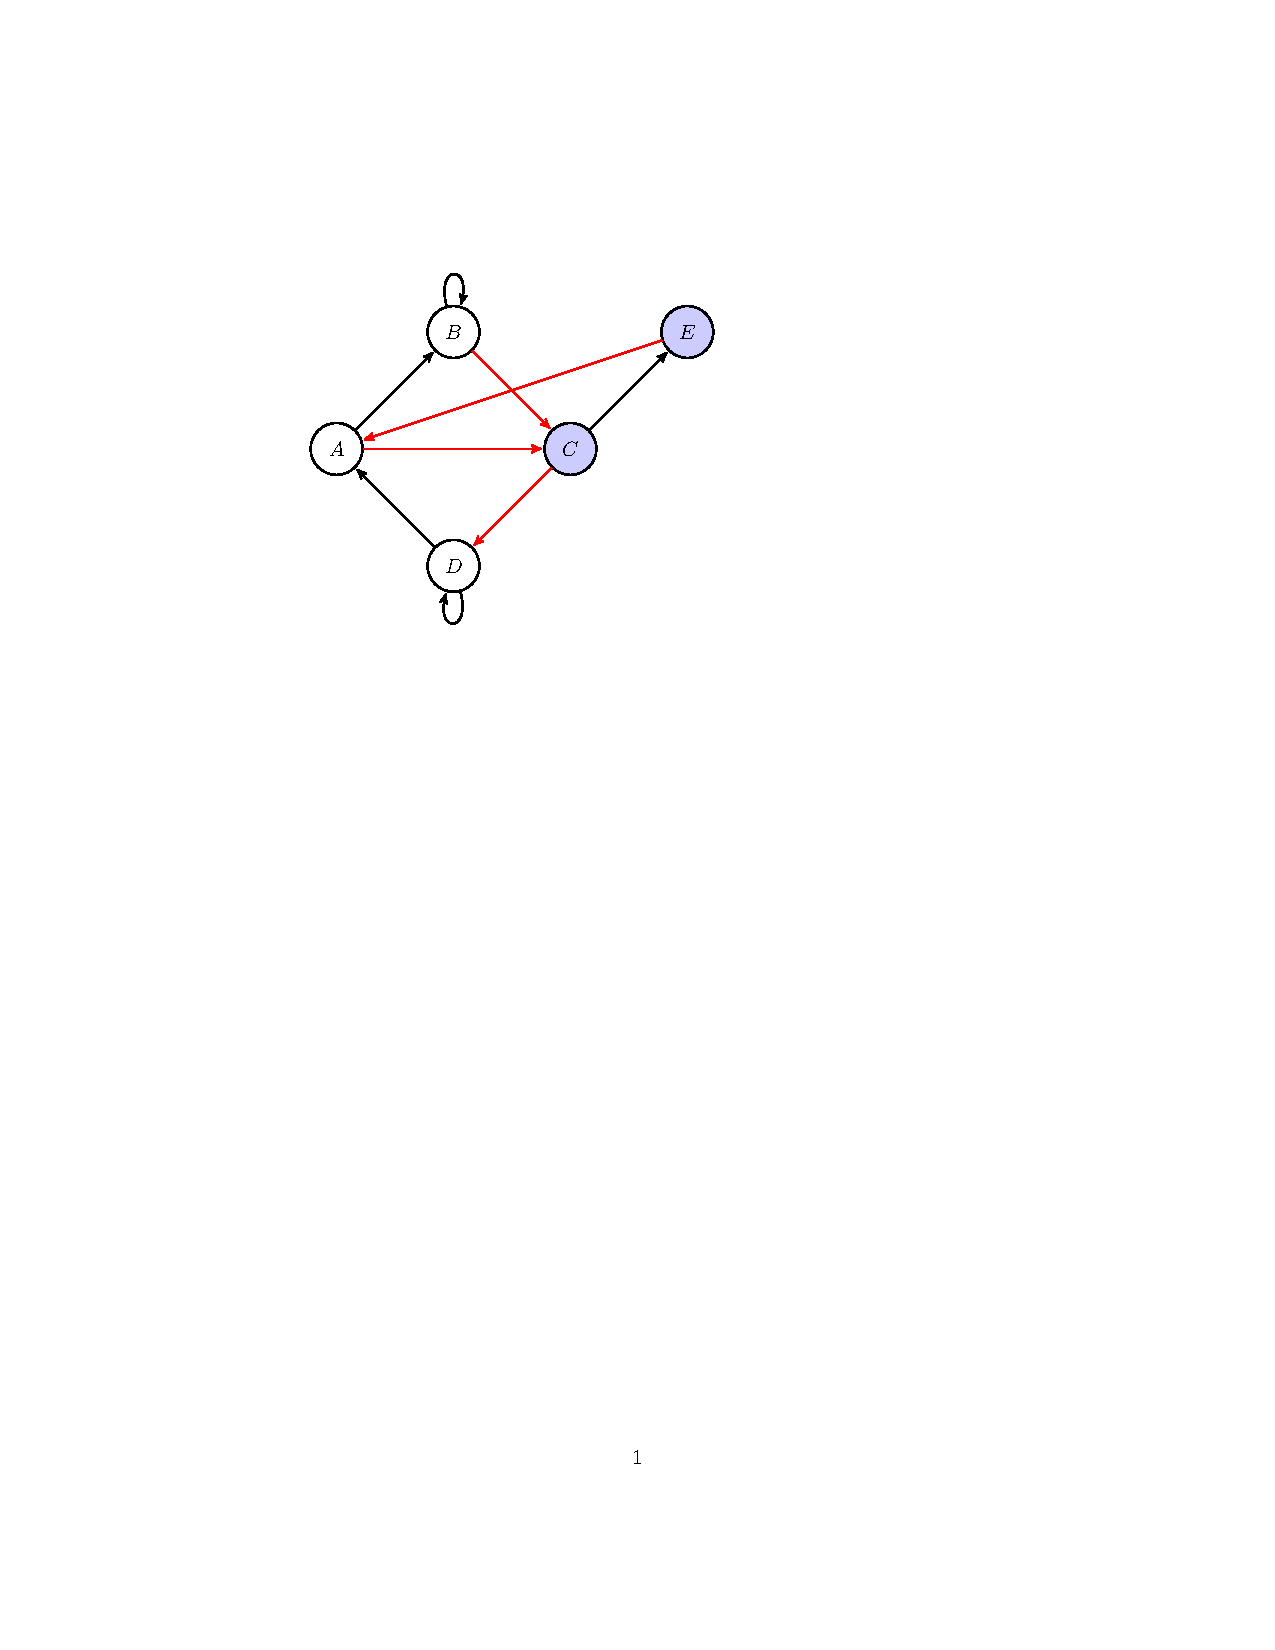
\includegraphics[width=.5\textwidth]{fund_conc/cut_example.pdf}
    \end{center}
    \caption{Grafo com exemplo de corte. O corte apresentado é definido
    pelos conjuntos de vertices ${E, C}$, em azul, e $A, B, D$, em 
    branco. Os arcos de cor vermelha são os arcos deste corte. No total,
    são 4 arcos vermelhos neste corte, ou seja, o tamanho deste corte
    é 4.}
    \label{fig:example_cut}
\end{figure}

Note que qualquer particionamento (não apenas bipartições) do conjunto 
de vértices de um grafo pode ser realizado após recursivas aplicações de 
cortes. Portanto, é possível construir e analisar cortes olhando apenas
para bipartições do grafo original. Perceba também que ao fazer um 
particionamento, podemos analisar o balanceamento de processamento 
dos nós de computação de acordo com o número de partes (e vértices) 
que são alocadas aos nós de computação. Além disso, é possível analisar
a quantidade de comunicação entre nós de acordo com a quantidade de
arestas que conectam diferentes partes (arestas de algum corte que), 
que podem estar alocadas em dois nós de computação diferentes.

{\color{blue} Se formos falar de cortes baseados em arestas, é melhor
adicionar mais um pedaço de texto explicando esse tipo de corte.}

\section{Particionamento de grafos}
% por que é importante?
% o que podemos analisar do grafo quando fazemos um particionamento
% - balanceamento
% - quantidade de links entre nós
% - e se quisermos levar em conta os nós que são mais acessados?
%   - pomos atualizar estas medidas com  pesos em arcos e nós.
% Quais são as principais abordagens para se fazer um particionamento?
\subsection{O algoritmo METIS}
\subsection{Particionamentos aleatórios}
\subsection{Particionamentos com semântica}

\section{Sistemas Gerenciadores de Bancos de Dados em Grafos}
\section{Graph Analytics Systems}
\subsection{Pregel}

\begin{thebibliography}{00}
\bibitem{nosqlorg} ``NoSQL Databases", http://nosql-database.org/.
\bibitem{neo4jcustomers} ``Neo4j Customers", https://neo4j.com/customers/.
\bibitem{neo4jquery} M. Hunger, R. Boyd. ``RDBMS \& Graphs: SQL vs. Cypher Query Languages" Neo4j Blog. Mar. 2016. https://neo4j.com/blog/sql-vs-cypher-query-languages/
\bibitem{biochem4j} N. Swainston et al., ``biochem4j: Integrated and extensible biochemical knowledge through graph databases,” PLOS ONE, vol. 12, no. 7, p. e0179130, Jul. 2017. 
\bibitem{biomol} F. Olken, ``Graph Data Management for Molecular Biology,” OMICS: A Journal of Integrative Biology, vol. 7, no. 1, pp. 75–78, Jan. 2003.
\bibitem{sematicweb} B. McBride, ``Jena: a semantic Web toolkit,” IEEE Internet Computing, vol. 6, no. 6, pp. 55–59, Nov. 2002.

\end{thebibliography}
\end{document}
